% 2010 年广东卷文科第 18 题：半圆 AEC 与三棱锥 F-BED。
% 来源 PDF：普通高考/2010/2010广东文.pdf，SHA-256 dd04b2053a22c854a9abe1ee03241fc04d5a25c91cda1d7997183bdfaa4a8c6f。
% 原页：第 2 页（A3 三栏）第 1 栏上部，书页码 596。
% 重绘依据：A、B、C、D 共线且 AB=BC=CD；半圆以 AC 为直径、E 为弧中点；
%   F 在 C 上方，FC⊥平面 BED。FC、FB 为不可见棱，画虚线。
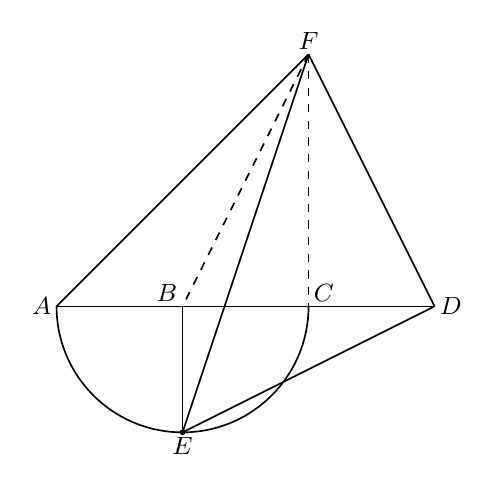
\begin{tikzpicture}[semithick, scale=0.8, every node/.style={inner sep=1.6pt, font=\small}]
  \coordinate (A) at (-2,0);
  \coordinate (B) at (0,0);
  \coordinate (C) at (2,0);
  \coordinate (D) at (4,0);
  \coordinate (E) at (0,-2);
  \coordinate (F) at (2,4);

  \draw (A) -- (D);
  \draw (A) arc[start angle=180,end angle=360,radius=2];
  \draw (F) -- (A);
  \draw (F) -- (D);
  \draw (F) -- (E);
  \draw[dashed] (F) -- (B);
  \draw[dashed] (F) -- (C);
  \draw (E) -- (B);
  \draw (E) -- (D);

  \fill (E) circle (1.3pt);
  \node[left] at (A) {$A$};
  \node[above left] at (B) {$B$};
  \node[above right] at (C) {$C$};
  \node[right] at (D) {$D$};
  \node[below] at (E) {$E$};
  \node[above] at (F) {$F$};
\end{tikzpicture}
